\documentclass[../../../../Lectures.tex]{subfiles}


\begin{document}

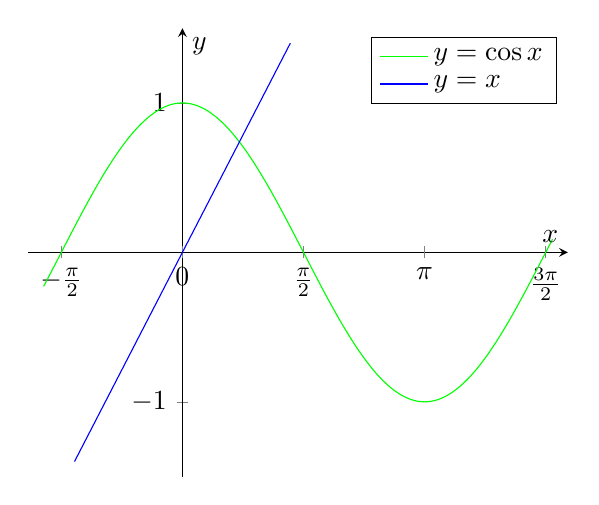
\begin{tikzpicture}
    \begin{axis}[
        axis lines=center,
        xlabel={\(x\)},
        xmin=-2, xmax=5,
        xtick=\empty,
        extra x ticks      ={-0.5 * pi         , 0, 0.5 * pi         , pi     , 1.5 * pi},
        extra x tick labels={\(-\frac{\pi}{2}\), 0, \(\frac{\pi}{2}\), \(\pi\), \(\frac{3 \pi}{2}\)},
        ylabel={\(y\)},
        ymin=-1.5, ymax=1.5,
        legend cell align={left},
    ]
        \addplot [green, samples=200, domain=-1.8:4.8] {cos(deg(x))};
        \addlegendentry{\(y = \cos{x}\)}

        \addplot [blue, samples=10, domain=-1.4:1.4] {x};
        \addlegendentry{\(y = x\)}
    \end{axis}
\end{tikzpicture}

\end{document}
